\documentclass[cs4size,a4paper,nofonts]{ctexart}
\def\titlee{矩阵乘法}
\CTEXsetup[number=\chinese{section}, name={,、}, format={\Large\bfseries}]{section}

\usepackage[utf8]{inputenc}
\def\tjf{{\tt{田劲锋}}}
\def\titlec{《算法设计与分析》综合性实验实验报告}
\usepackage[top=2.54cm,bottom=2.54cm,left=3.17cm,right=3.17cm]{geometry} % 页面设置
\usepackage[unicode,breaklinks=true,
colorlinks=true,linkcolor=black,anchorcolor=black,citecolor=black,urlcolor=black,
pdftitle={\titlec},pdfauthor={\tjf}]{hyperref}
\usepackage{tikz} % 画图
\usetikzlibrary{shapes,arrows}
\usepackage{multicol} % 分栏
\usepackage{multirow} % 跨行
\usepackage{longtable} % 长表格
\usepackage{tabularx} % 变宽表格
\usepackage{booktabs} % 表格画线
\usepackage{graphicx} % 图形
\usepackage{color} % 颜色
\usepackage{xcolor} % 颜色
\usepackage{wallpaper} % 背景图片
\usepackage{listings} % 排版代码
\lstset{language=C++,
  numbers=left,
  numberstyle=\tiny,
  basicstyle=\small\tt,
  commentstyle=\color{gray},
  keywordstyle=\bfseries\color{violet},
  stringstyle=\color{teal},
  showstringspaces=false,
}
\usepackage{amsmath,bm}
\usepackage{verbatim} % 排版代码
\usepackage{url} % 排版链接
\usepackage{shortvrb}
\usepackage{pstricks} % 绘图
\usepackage{pst-tree} % 画树
% \usepackage{pst-uml} % 画 UML
\usepackage{uml} % 画 UML
\usepackage{clrscode3e} % CLRS 伪代码
\usepackage{smartdiagram} % 智能画图
\usepackage{nameref}
\usepackage{rotating} % 横排大图
\usepackage{caption}
\captionsetup{font={small}} % 标题字体大小
\usepackage[inline]{enumitem} % 调整列表样式

%\setmainfont{Times New Roman}
\setCJKmainfont[BoldFont={SimHei}]{SimSun}  % 主要字体:宋体、黑体
\setCJKsansfont[BoldFont={STZhongsong}]{STFangsong} % 次要字体:仿宋、中宋
\setCJKmonofont{KFKai} % 等宽字体:楷体
\setCJKfamilyfont{msyh}[BoldFont={* Bold}]{微软雅黑} \newcommand{\msyh}{\CJKfamily{msyh}} % 微软雅黑
\setCJKfamilyfont{micro}{文泉驿微米黑} \newcommand{\micro}{\CJKfamily{micro}} % 文泉驿微米黑
\setCJKfamilyfont{yaoti}{方正姚体} \newcommand{\yaoti}{\CJKfamily{yaoti}}

\CJKsetecglue{\hspace{0.1em}}
\renewcommand\CJKglue{\hskip -0.3pt plus 0.08\baselineskip}
\frenchspacing
\widowpenalty=10000
\linespread{1.5} % 1.5 倍行距
\setlength{\parskip}{2pt plus 2pt}
\renewcommand{\baselinestretch}{1.5}

\setlength{\abovecaptionskip}{1pt}
\setlength{\belowcaptionskip}{0pt}
\setlength{\intextsep}{8pt}

\makeindex
\pagestyle{plain}


\begin{document}
\begin{titlepage}

\begin{center}


\includegraphics[height=1cm]{image/haut.png}

\vspace*{1cm}
{\liti\fontsize{48pt}{50pt}{课\quad 程\quad 设\quad 计}}

\vspace*{4cm}
{\fontsize{36}{80}\sf\bfseries \titlec}

\vspace*{1cm}
{\fontsize{30}{70}\sf\bfseries \titlee}

\vfill
{\large
\newcommand{\ctline}[2]{\makebox[6em][s]{\bf #1}:\underline{\makebox[14em][c]{\qquad #2\qquad}}\\}
\ctline{课程设计名称}{数据结构课程设计}
\ctline{专业班级}{计算机 1303 班}
\ctline{学生姓名}{\tjf}
\ctline{学号}{201316920311}
\ctline{指导教师}{白\quad 浩}
\ctline{课程设计时间}{\today}
}

\end{center}

\end{titlepage}
\newpage

\section{实验题目}
矩阵乘法
\section{实验目的}
\begin{enumerate}[topsep=0pt,partopsep=0pt,itemsep=0pt,parsep=0pt]
\item 掌握二维数组的使用方法。 
\item 掌握文件的读入和输出。 
\item 掌握复杂循环的设计方法。
\end{enumerate}
\section{实验要求}
任给两个矩阵$\bm A$和$\bm B$,计算它们的乘法。

具体要求:

(1)每个矩阵输入的格式如下:第一行的两个数字分别表示行$n$和列$m$,随后紧跟包含$m$列的$n$行来表示矩阵。将两个输入矩阵保存在input.txt文件中。举例如下:
\begin{quote}
\verbatiminput{alys01/input.txt}
\end{quote}

(2)将两个矩阵的运算结果保存在文件output.txt中。

\section{程序流程图}

设$\bm A = (a_{ij})_{m \times s}$, $\bm B = (b_{ij})_{s \times n}$,
矩阵乘法定义为$$\bm C=\bm A  \bm B,$$
其中 $$\bm C=(c_{ij})_{m\times n},$$
$$c_{ij} = a_{i1}b_{1j} + a_{i2}b_{2j} + \cdots + a_{is}b_{sj}
= \sum_{k=1}^{s}{a_{ik}b_{kj}}.$$

可以得出矩阵乘法的算法,伪代码如图\ref{mul}。
\begin{figure}[htp]
\begin{quote}
\begin{codebox}
\Procname{\proc{Matrix::$\times$}($A, B$)}
\li $C.l = A.l$
\li $C.c = B.c$
\li \For $i = 1$ \To $A.l$ \Do
\li   \For $j = 1$ \To $B.c$ \Do
\li     \For $k = 1$ \To $A.c(=B.l)$ \Do
\li       $C[i][j] = A[i][k]\times B[k][j]$
        \End
      \End
    \End
\li \Return $C$
\end{codebox}
\end{quote}
\caption{\label{mul}矩阵乘法的算法}
\end{figure}

二维数组的输入输出则是比较简单的,流程图\ref{f1}描述了二维数组的输入过程。
\begin{figure}[htp]
\centering
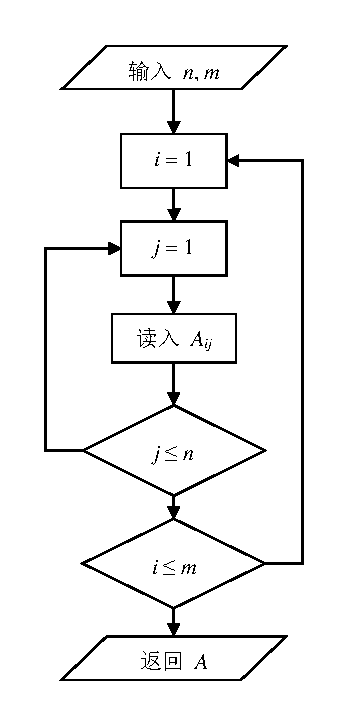
\includegraphics[height=10cm]{alys01/f1.pdf}
\caption{\label{f1}矩阵输入过程}
\end{figure}

输出同理,不再赘述。

\section{程序代码}
{\linespread{1}\lstinputlisting{alys01/alys01.cpp}}

\section{实验结果}
输出文件output.txt:
\begin{quote}
\verbatiminput{alys01/output.txt}
\end{quote}

实际上该样例即是此式:
\[
\left[\begin{array}{ccc}
1 & 2 & 3\\
4 & 5 & 6\\
7 & 8 & 9
\end{array}\right]
\cdot
\left[\begin{array}{c}
1\\
1\\
1
\end{array}\right]
=
\left[\begin{array}{c}
   6\\
  15\\
  24
\end{array}\right]
\]

\section{实验体会}
这道题目比较适合用于练手,虽然简单但是也有一些细节需要仔细处理。结合最近学习的C++课程,我使用了简单的类来实现这个矩阵乘法的题目。实际上这个程序还不能很好地表现OOP的精髓,比如输入输出逻辑绑定在了类中,应该另外做一个接口的。文件的输入输出则简单的使用了文件重定向,也可在命令行下使用重定向符来重定向输入输出流。

关于程序流程图的问题,我觉得在一定程度上,这个流程图是个累赘,描述算法还是伪代码比较合适。

本来打算用Word随便做做交了的,想到老师实验课上严重的\TeX 痕迹,那就换成\TeX 来排版了。虽然是驾轻就熟的工具,但是改改模板还是费点心思的。

\end{document}
